
\section{Smoothed canonicalization} \label{appendix:canon}

\noindent
This appendix expands on the discussion in \cref{sec:canon} and \cref{sec:symm:inference}. We restrict our attention to a diagonal group $\Gdiag$ induced by a space group $\G=\G_{\rm sp}$. 

\vspace{.5em}

The essential idea behind canonicalization is that, to construct an invariant layer under $\Gdiag$, one may perform a ``projection" onto a ``smallest invariant set'' $\Pi \subset \R^{3n}$, called the fundamental region. Formally, $\Pi$ is a fixed set that contains exactly one point from each orbit of $\G_\diag$ -- called the \emph{representative} point of the orbit -- and canonicalization is an $\R^{3n} \rightarrow \Pi$ map that brings an input $x$ to its corresponding representative. In the simple case of unit translations and $n=1$, a standard canonicalization is $x \mapsto  x\;{\rm mod}\;1$ with $\Pi = [0,1)$, as visualized in Fig.~\ref{fig:canon:1d}. A naive canonicalization suffers from boundary discontinuity that violates physical constraints: In the case of ${\rm mod}$, this arises because
\begin{align*}
    \textstyle\lim_{\epsilon \rightarrow 0^+} (\epsilon\,{\rm mod}\,1) 
    = 0 \neq 1 = 
    \textstyle\lim_{\epsilon \rightarrow 0^-} (\epsilon\,{\rm mod}\,1)\;.
    \tagaligneq \label{eq:1d:discontinuity}
\end{align*}
Resolving this requires introducing smoothing at the boundary. As an example, consider the supercell assumption \citep{rajagopal1995variational,kittel2018introduction}, which corresponds to separate invariance under translations along each 1d lattice vector. Jastrow factors (\cite{whitehead2016jastrow}; also see \cite{li2022ab} for its implementation in DeepSolid) exactly perform a smoothed version of canonicalization along each 1d lattice vector: These factors take the form $h(x \, {\rm mod} \, 1)$, where $x \in \R$ is a suitably rescaled input along one lattice vector and $h$ is a piecewise polynomial chosen such that $x \,\mapsto\, h(x \, {\rm mod} \, 1)$ is twice continuously differentiable. However, the construction of $h$ is easy here only because the fundamental regions of 1d translations have simple boundaries (two endpoints), and does not generalize well to more complicated symmetries. 

\vspace{.5em}

For groups such as permutations and rotations, \citet*{dym2024equivariant} proposes a smoothing method by taking weighted averages at the boundary. We adapt this method for our $\Gdiag$ induced by a space group, and show how it can be achieved by operating with the group $\G$ acting on single electrons. This requires two ingredients:

\begin{itemize}
    \item \textbf{Fundamental region of $\Gdiag$.} There are infinitely many choices of fundamental regions, and we shall fix one that is convenient for our canonicalization. Fix $\Pi_0 \subset \R^3$, a fundamental region of $\R^3$ under $\G$. Then $\Pi \coloneqq \Pi_0 \times (\R^3)^{n-1}$ forms a fundamental region under $\Gdiag$, as it is intersected exactly once by any orbit $\{ (g(x_1), \ldots, g(x_n)) \,|\, g\in \G\}$. An advantage of this choice is that, since the boundary of $\Pi $ is completely determined by the boundary of $\Pi_0$ in the space of the first electron, we may perform smoothing directly near the boundary of $\Pi_0$. Also notice that we may equivalently choose the fundamental region $\Pi^{(k)} \coloneqq (\R^3)^{k-1} \times \Pi_0 \times (\R^3)^{n-k-1}$ for any $1 \leq k \leq n$.
    \item \textbf{Smoothing factor.} Fix some small $\epsilon > 0$. For each $x \in \R^3$, consider the set of group elements that moves $x$ to be at most $\epsilon$-away from $\Pi_0$:
    \begin{align*}
        \cG_\epsilon(x) 
        \;\coloneqq\;
        \big\{ g \in \G \,\big|\, d( g(x), \Pi_0) \leq \epsilon \big\}
        \;,
    \end{align*}
    where $d$ is some distance preserved by the isometries in $\G$:
    \begin{align*}
        d( g(x), g(\Pi_0) ) \;=\; d( x, \Pi_0 )
        \; \text{ for all } g \in \G \text{ and } x \in \R^3\;.
    \end{align*}
    Adapting the weighted averaging idea from \citet{dym2024equivariant}, we perform smoothing in the $\epsilon$-neighborhood of $\Pi_0$ by assigning weights to the different group operations: For each $g \in \G$, we define 
    \begin{align*}
        w^g_\epsilon(x) \;\coloneqq\; \mfrac{ \lambda_\epsilon( \, d(g(x), \Pi_0) \,  )}{\sum_{g' \in \cG_\epsilon(x)} \, \lambda_\epsilon( \, d(g'(x), \Pi_0) \,)  }
        \;\in\; [0,1]
        \;,
    \end{align*}
    where $\lambda_\epsilon: \R \rightarrow [0,1]$ is a strictly decreasing function such that $\lambda_\epsilon(w) = 1$ for all $w \leq 0$ and $\lambda_\epsilon(w) = 0$ for all $w \geq \epsilon$. If $d(g(x), \Pi_0) \geq \epsilon$, $g$ moves $x$ ``too far'', and is assigned zero weights. If $d(g(x), \Pi_0) = 0$, $g$ keeps $x$ within the closure of $\Pi_0$, and is assigned a weight of $1$. In particular, if $x \in \Pi_0$ is a point of high symmetry and $\epsilon$ is small enough such that $g(x)=x$ for all $g \in \cG_\epsilon(x)$, the weight of every $g \in \cG_\epsilon(x)$ is $\frac{1}{|\cG_\epsilon(x)|}$: Here, all operations that preserve $x$ are assigned equal weights. See \cref{appendix:lambda:d} for explicit choices o $d$ and $\lambda_\epsilon$.
\end{itemize}

\vspace{.5em}

With these tools at hand, we define the smoothed canonicalization (SC) of an unsymmetrized wavefunction $f_\theta$ as 
\begin{align*} 
    \psiSC_{\theta;\epsilon}(\bx)
    \;\coloneqq\;
    \mfrac{1}{n} 
    \msum_{k=1}^n
    \psiSCk_{\theta;\epsilon}
    (\bx)
    \;,
    \qquad 
    \text{ where }
    \quad
    \psiSCk_{\theta;\epsilon}
    (\bx)
    \;\coloneqq\; 
    \msum_{g \in \cG_\epsilon(x_k)} 
    w^g_\epsilon(x_k)
    \, \psi_\theta( g(\bx))
    \;.
    \tagaligneq 
    \label{eq:SC}
\end{align*}
\cref{appendix:SC:illustration} illustrates \eqref{eq:SC} through an one-electron example. The next result guarantees the validity of $\psiSC_{\theta;\epsilon}(\bx) = \frac{1}{n} \sum_{k=1}^n \psiSCk_{\theta;\epsilon}(\bx)$ as a symmetrized wavefunction: \cref{thm:SC}(i) proves diagonal invariance, (ii) proves anti-symmetry and (iii) ensures smoothness under appropriate choices of $\lambda_\epsilon$ and $d$.


\begin{theorem} \label{thm:SC} Fix $\theta \in \R^q$ and $\epsilon > 0$.  The following properties hold for $\psiSC_{\theta;\epsilon}$ and $\psiSCk_{\theta;\epsilon}$ for all $1 \leq k \leq n$:
\begin{enumerate}
    \item[(i)] $\psiSCk_{\theta;\epsilon}(g(\bx)) =  \psiSCk_{\theta;\epsilon}(\bx)$ for all $g \in \G$ and $\bx \in \R^{3n}$;
    \item[(ii)] Let the spin-dependence in $\psi_\theta$ be explicit, i.e.~we view $\psi_\theta$ as an $(\R^3 \times \{\uparrow, \downarrow \})^n \rightarrow \C$ function. If $\psi_\theta$ is anti-symmetric with respect to permutations of $(x_i, \sigma_i)$, then so is $\psiSC_{\theta;\epsilon}$;
    \item[(iii)] Suppose $\lambda_\epsilon$ and $d(\argdot, g(\Pi_0))$ are $p$-times continuously differentiable for all $g \in \G$, and that $\psi_\theta$ is $p$-times continuously differentiable at $g(\bx) \in \R^{3n}$ for all $g \in \G$. Then $\psiSC_{\theta;\epsilon}$ is also $p$-times continuously differentiable at $\bx$. Moreover for $0 \leq q \leq p$, the $q$-th derivative of $\psiSC_{\theta;\epsilon}$ at $\bx=(x_1, \ldots, x_n)$ can be computed as 
        \begin{align*}
            \nabla^q 
            \psiSC_{\theta;\epsilon}(x_1, \ldots, x_n)
            \;=&\;
            \mfrac{1}{n}
            \msum_{k=1}^n
            \msum_{g \in \cG_\epsilon(x_k)}
            \,
            \nabla^q 
            \psiSCk_{\theta,\epsilon;g,x_k}
            (\bx)\;,
        \end{align*}
        where we have defined, for $1 \leq k \leq n$, $g \in \G$ and $x, y_1, \ldots, y_n \in \R^3$, 
        \begin{align*}
            \psiSCk_{\theta,\epsilon;g,x}
            (y_1, \ldots, y_n)
            \;\coloneqq&\;
            \mfrac{
                \lambda_\epsilon
                \big( d( y_k, g(\Pi_0) \big) \big) 
            }{
                \sum_{g' \in \cG_\epsilon(x)}
                \lambda_\epsilon
                \big( d( y_k, g'(\Pi_0) \big) \big) 
            }
            \,
            \psi_\theta( g^{-1}(y_1) \,,\, \ldots \,,\, g^{-1}(y_n) )
            \;.
        \end{align*}
\end{enumerate}   
\end{theorem}

\noindent
\textbf{Computational cost compared to DA and GA.} As mentioned in \cref{sec:canon}, SC suffers from a similar computational issue as DA and GA as it involves averaging. However, the amount of averaging SC requires is different. The additional averaging over $n$ fundamental regions is crucial for ensuring anti-symmetry, which is made precise in \cref{thm:SC} and its proof in \cref{appendix:proof:canon}. Averaging is also required over the set $\cG_\epsilon$, which necessarily includes all point group operations and unit translations of $\G$ (note that $\cG_\epsilon$ is not a group). For a fair comparison, compare SC to DA and GA that average over the group $\G$. For small systems with $1 \times 1 \times 1$ supercell, $\cG_\epsilon$ is strictly larger than the point group $\G$, and the amount of averaging required by SC, $n |\cG_\epsilon|$, is strictly larger. For large systems, the cost of SC scales differently from DA and GA: While the cost of DA and GA increase as a function of the increasing group size $|\G|$, for SC, $\cG_\epsilon$ is fixed and the cost increases as a function of the number of electrons $n$.

\vspace{.5em}

\noindent
\textbf{Post hoc smoothed canonicalization (PC).} As discussed in \cref{sec:symm:inference}, we may perform canonicalization only at evaluation. However, there is an inherent tradeoff in the choice of $\epsilon$: If $\epsilon$ is large, averaging happens in a large neighborhood of the boundary, which can cause the performance of $\psi^{(\rm SC)}_{\hat \theta;\epsilon}$ to deviate significantly from the well-trained $\psi^{(\rm OG)}_{\hat \theta}$ (see \cref{appendix:SC:illustration}). If $\epsilon$ is small, there may be a blowup in the derivatives of the weights via the smoothing function:

% A notable difference is that we can now take advantage of the fact that $\psiSC_\theta$ is completely determined by the value of $\psi_\theta$ on $\Pi_\epsilon$, an appropriately defined $\epsilon$-neighborhood of $\cup_{k \leq n} \Pi^{(k)}$. 


\begin{lemma} \label{lem:eps:lamb:blowup} If $\lambda_\epsilon$ is twice continuously differentiable, there are $y_1, y_2 \in [0, \epsilon]$ s.t.~$\partial \lambda_\epsilon(y_1) = \epsilon^{-1}$, $\partial^2 \lambda_\epsilon(y_2) = \epsilon^{-2}$.
\end{lemma}


Since the local energy calculation involves $\partial^2 \lambda_\epsilon$, this can lead to an $\epsilon^{-2}$ blowup of local energy in a region of size $O(\epsilon)$, resulting in larger fluctuations of local energy. This inflation in the variance is clearly visible in \cref{table:stats}.


% \color{blue} \khh{PAUSE - TO REWRITE}
% i.e.~the union of the fundamental regions with different reference electrons. In other words, $\hat \theta$ only needs to be trained to perform well on $\Pi_\epsilon$. 
% Let $P_{\Pi_\epsilon}: \R^{3n} \rightarrow \R^{3n}$ be the projection operator onto $\Pi$. We propose to train the ``projected" network $\psi_\theta \circ P_{\Pi_\epsilon}$, and show in \cref{appendix:projected:SC} that for first-order methods, this is equivalent to using the parameter update rule 
% \begin{align*}
%     \theta 
%     \;\mapsto&\,\;
%     \theta \,-\, \mean_{\bX \sim p_{\psi_\theta}}[ F_{ P_{\Pi_\epsilon}(\bX);\psi_\theta} ]
%     \;,
% \end{align*}
% i.e.~training $\psi_\theta \circ P_{\Pi_\epsilon}$ is the same as training the original network $\psi_\theta$ on samples that are projected through $P_{\Pi_\epsilon}$. A similar result also holds for second-order methods. Having obtained the converged parameter $\hat \theta$, at evaluation, we then sample from the full smoothed canonicalization $f_{\hat \theta}^{(\rm SC)}$.

% Two issues persist in the post hoc canonicalization setup: 

% \khh{PAUSE - TO-REARRANGE}


% Another issue is fundamental to $\psiSC_{\theta;\epsilon}$: If $\epsilon$ is large, undesired additional symmetries can appear (see \cref{appendix:SC:epsilon:large}), whereas if $\epsilon$ is small, there may be a blowup in the derivatives of the weights via the smoothing function:


\subsection{Choices of $\lambda_\epsilon$ and $d$} \label{appendix:lambda:d}


\begin{figure}[t]
    \centering
    \begin{tikzpicture}
        \node[inner sep=0pt] at (0,0) {\includegraphics[trim={0 1.2em 0 0.5em},clip,width=\linewidth]{figs/lambda_plot.pdf}};
    \end{tikzpicture}   
    \vspace{-1.8em}
    \caption{Illustration of different choices of step functions $s$, the corresponding $\lambda_\epsilon$'s and their first two derivatives. $\epsilon=0.1$ above.}
    \label{fig:lambda}
    \vspace{-1em}
\end{figure}


To obtain a $p$-times continuously differentiable $\psi^{(\rm SC)}_{\theta,\epsilon}$, \cref{thm:SC}(iii) requires a smoothing function $\lambda_\epsilon$ and a distance function $d(\argdot, g(\Pi_0))$ that are $p$-times continuous differentiable for all $g \in \G$.

\vspace{.5em}

\noindent
\textbf{Construction of $\lambda_\epsilon$.} Since $\lambda_\epsilon: \R \rightarrow [0,1]$ is required to be strictly decreasing with $\lambda_\epsilon(w) = 1$ for $w \leq 0$ and $\lambda(w)=0$ for all $w \geq \epsilon$, the function 
\begin{align*}
    s(w) \;\coloneqq\; \lambda_\epsilon( \, \epsilon( 1 - w) \, )
\end{align*}
is a $p$-times continuously differentiable approximation of a step function: $s$ is strictly increasing, $s(w) = 0$ for all $w \leq 0$ and $s(w) = 1$ for all $w \geq 1$. Many choices are available for such a function: To have an infinitely differentiable $\lambda_\epsilon$, one may consider the smoothed step function
\begin{align*}
    s_\infty(w) \;\coloneqq\; \mfrac{ \phi(w) }{ \phi(w) + \phi(1-w)}
    \qquad 
    \text{ where }
    \phi(w ) \;\coloneqq\; \begin{cases}
        \exp(- w^{-1}) & \text{ if } w > 0 \;,
        \\
        0 & \text{ if } w \leq 0 \;,
    \end{cases}
\end{align*}
and use the relationship $\lambda_\epsilon(w) = s\big(  1 - w / \epsilon \big)$ to obtain
\begin{align*}
    \lambda_{\epsilon;\infty}(w) 
    \;\coloneqq\;
    \mfrac{ \phi(1 - w / \epsilon) }{ \phi( 1 - w/\epsilon) + \phi(w / \epsilon)}
     \;.
\end{align*}
As we only need to evaluate the Hamiltonian, twice continuous differentiability typically suffices for our problem. Another choice of the step function $s$ and the corresponding $\lambda_\epsilon$ are the degree-three polynomial splines
\begin{align*}
    s_2(w) \;\coloneqq\; 
    \begin{cases}
        0 & \text{ if } w \leq 0\;, 
        \\
        \frac{9w^3}{2} & \text{ if } w \in (0,\frac{1}{3}]\;, 
        \\
        - \frac{9(1-w)^3}{2} + \frac{(2-3w)^3}{2} + 1 & \text{ if } w \in (\frac{1}{3},\frac{2}{3}]\;, 
        \\
        - \frac{9(1-w)^3}{2} + 1 & \text{ if } w \in (\frac{2}{3},1]\;, 
        \\
        1 & \text{ if } w > 1 \;,
    \end{cases}
    \;\;
    \lambda_{\epsilon;2}(w) \;\coloneqq\; 
    \begin{cases}
        1 & \text{ if } w \leq 0\;, 
        \\
        1 - \frac{9w^3}{2\epsilon^3} & \text{ if } w \in (0,\frac{\epsilon}{3}]\;, 
        \\
        - \frac{9 w^3}{2 \epsilon^3} + \frac{(3w - \epsilon )^3}{2 \epsilon^3} + 1  & \text{ if } w \in (\frac{\epsilon}{3},\frac{2\epsilon}{3}]\;, 
        \\
        \frac{9(\epsilon - w)^3}{2 \epsilon^3}  & \text{ if } w \in (\frac{2\epsilon}{3}, \epsilon]\;, 
        \\
        0 & \text{ if } w > \epsilon \;,
    \end{cases}
\end{align*}
Fig.~\ref{fig:lambda} plots $s_\infty$, $s_2$, $\lambda_{\epsilon;\infty}$, $\lambda_{\epsilon;2}$ and their derivatives. Note that the derivative plots for $\lambda_\epsilon$'s verify \cref{lem:eps:lamb:blowup}. To achieve general $p$-times continuous differentiability, we refer readers to the many constructions of such step functions available in the statistics literature, e.g.~Theorem 3.3 of \citet{chen2011normal} or Lemma 34 of \citet{huang2023high}. In particular, our $s_2$ is related to $h_{m;\tau;\delta}$ constructed in Lemma 34 of \citet{huang2023high} via $s_2(w) = h_{2;1;1}(w)$; one can similarly take their $h_{p;1;1}$ to obtain a $p$-times continuously differentiable $s_p$ and obtain the corresponding $\lambda_{\epsilon;p}(w) \coloneqq 1 - s_p(w/\epsilon)$.


\begin{figure}[t]
    \centering
    \begin{tikzpicture}
        \node[inner sep=0pt] at (0,0) {\includegraphics[width=\linewidth]{figs/weights_1d.pdf}};
        \node[inner sep=0pt] at (.35, 5.8) {\footnotesize $\epsilon = 0.1$};
        \node[inner sep=0pt] at (-5.05, 5.8) {\footnotesize $\epsilon = 0.001$};
        \node[inner sep=0pt] at (5.8, 5.8) {\footnotesize $\epsilon = 0.5$};
    \end{tikzpicture}   
    \vspace{-1.8em}
    \caption{Plots of $\tilde w_\epsilon(x-1)$, $\tilde w_\epsilon(x)$ and $\tilde w_\epsilon(x+1)$ defined via either $s_\infty$ or $s_2$ as the smoothed step function used in $\lambda_\epsilon$ and $d$, and for different values of $\epsilon$. }
    \label{fig:weight:1d}
\end{figure}
\begin{figure}[t]
    \centering
    \begin{tikzpicture}
        \node[inner sep=0pt] at (0,0) {\includegraphics[width=\linewidth]{figs/weights_grad_1d.pdf}};
        \node[inner sep=0pt] at (-5.05, 3.9) {\footnotesize $\epsilon = 0.001$};
        \node[inner sep=0pt] at (.35, 3.9) {\footnotesize $\epsilon = 0.1$};
        \node[inner sep=0pt] at (5.8, 3.9) {\footnotesize $\epsilon = 0.5$};
    \end{tikzpicture}   
    \vspace{-2em}
    \caption{Plots of derivatives of $\tilde w_\epsilon(x)$ for different values of $\epsilon$. }
    \label{fig:weight:gradient:1d}
\end{figure}

\vspace{.5em}

\textbf{Constructing $d(\argdot, g(\Pi_0))$ via the step function $s$.} A $p$-times continuously differentiable step function $s$, as discussed above, induces a $p$-times continuously differentiable approximation of ${\rm max}\{ \argdot, 0 \}$, given as 
\begin{align*}
    \tilde s(w) \;\coloneqq\; w \, s(w)\;.
\end{align*}
In particular $\tilde s(w) =0 $ if and only if $w \leq 0$, and $\tilde s(w) = w$ for $w \geq 1$. To utilize $\tilde s$ to construct $d(\argdot, g(\Pi_0))$, we notice that each $g(\Pi_0)$ itself is a fundamental region, and its closure is a simplex completely characterized by the relation
\begin{align*}
    x \in g(\Pi_0) \;\Leftrightarrow\; \mfrac{(x - g(c_0))^\top n_l}{\| n_l \|^2} \leq 1 \text{ for } 1 \leq l \leq m \;, 
\end{align*}
where $c_0$ is the center of $\Pi_0$ and $n_l$ is the normal vector starting from $c_0$ that is normal to the $l$-th face of $\Pi_0$. This allows us to define 
\begin{align*}
    d(x, g(\Pi_0)) \;\coloneqq\; 
    \msum_{l=1}^m  
    \Big( 
        \tilde s \Big( \mfrac{(x - g(c_0))^\top n_l}{\| n_l \|^2}  -1 \Big) 
    \Big)^2
    \;.
\end{align*}
This distance function satisfies that 
\begin{itemize}
    \item $ d(g(x), g(\Pi_0)) = d(x, \Pi_0)$ for all $g \in \G$, which can be verified by noting that $g(\argdot) = A(\argdot) + b$ for an orthogonal matrix $A \in \R^{3 \times 3}$ and a translation vector $b \in \R^3$;
    \item $d(x, \Pi) = 0$ if and only if $x \in \Pi$, and the map $x \mapsto d(x,\Pi)$ is $p$-times continuously differentiable. 
\end{itemize}
To visualize this distance function in the case of a 1d system, see Fig.~\ref{fig:dist:1d}.

\subsection{An one-electron example of $\psiSC_{\theta;\epsilon}$} \label{appendix:SC:illustration}

\begin{figure}[t]
    \vspace{.5em}
    \centering
    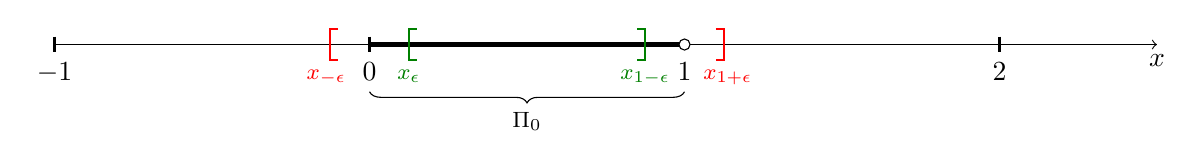
\begin{tikzpicture}
        \pgfmathsetmacro{\xzero}{-2.0}   
        \pgfmathsetmacro{\xdist}{4.0}   
        \pgfmathsetmacro{\xminusone}{\xzero-\xdist}   
        \pgfmathsetmacro{\xone}{\xzero+\xdist}   
        \pgfmathsetmacro{\xtwo}{\xzero+2*\xdist}   

        % Draw the x-axis
        \draw[->] (-6,0) -- (8,0) node[anchor=north] {$x$};

        \draw[-,ultra thick] (\xzero,0) -- (\xone,0);

        \draw[black!50!green,thick] (-1.4,0.2) -- (-1.5,0.2) -- (-1.5,-0.2) -- (-1.4,-0.2);
        \node[below,black!50!green] at (-1.5,-0.2) {\footnotesize $x_\epsilon$};

        \draw[red,thick] (-2.4,0.2) -- (-2.5,0.2) -- (-2.5,-0.2) -- (-2.4,-0.2);
        \node[below,red] at (-2.55,-0.2) {\footnotesize $x_{-\epsilon}$};

        \draw[black!50!green,thick] (1.4,0.2) -- (1.5,0.2) -- (1.5,-0.2) -- (1.4,-0.2);
        \node[below,black!50!green] at (1.5,-0.2) {\footnotesize $x_{1-\epsilon}$};

        \draw[red,thick] (2.4,0.2) -- (2.5,0.2) -- (2.5,-0.2) -- (2.4,-0.2);
        \node[below,red] at (2.55,-0.2) {\footnotesize $x_{1+\epsilon}$};

        % Marker at x = 0
        \draw[thick] (\xzero,0.1) -- (\xzero,-0.1) node[anchor=north] {$0$};
        
        % Marker at x = 1
        \filldraw[fill=white, draw=black] (\xone,0) circle (.2em);

        \node[below] at (\xone,-0.1) {$1$};

        \draw[thick] (\xminusone,0.1) -- (\xminusone,-0.1) node[anchor=north] {$-1$};
        \draw[thick] (\xtwo,0.1) -- (\xtwo,-0.1) node[anchor=north] {$2$};

        \draw[decorate, decoration={brace, mirror, amplitude=4pt}] (\xzero,-0.6) -- (\xone,-0.6)
        node[midway, below=4pt] {\footnotesize $\Pi_0$};

    \end{tikzpicture}
    \vspace{-.8em}
    \caption{Illustration of smoothed canonicalization $\psiSC_{\theta;\epsilon}$ for a single 1d electron}
    \label{fig:psiSC:1d}
\end{figure}

\begin{figure}[t]
    \vspace{-.5em}
    \centering
    \begin{tikzpicture}
        \node[inner sep=0pt] at (-5.5,0) {\includegraphics[width=\linewidth]{figs/dist_plot.pdf}};
    \end{tikzpicture}   
    \vspace{-2.5em}
    \caption{Plots of $d(x,[0,1))$ and its derivatives under different choices of the step function $s$.}
    \label{fig:dist:1d}
\end{figure}

For simplicity, we first illustrate $\psiSC_{\theta;\epsilon}$ for a single 1d-electron system with unit translation invariance. In this case, the group $\G$ is generated by translations of length 1, and the fundamental region is $\Pi_0 = [0,1)$, as illustrated in Fig.~\ref{fig:psiSC:1d}. As discussed at \eqref{eq:1d:discontinuity}, a standard canonicalization is to take $x \mapsto x \,{\rm mod}\, 1$, which suffers from discontinuity at the boundary. Our proposed smoothed canonicalization in this case becomes 
\begin{align*}
    \psiSC_{\theta;\epsilon}(x) 
    \;=\; 
    \msum_{t \in \Z \textrm{ s.t. }  d(x+t, [0,1))} 
    \,
    \mfrac{ \lambda_\epsilon\big( d(x+t, [0,1)) \big)}{\sum_{t' \in \Z \textrm{ s.t. }  d(x+t', [0,1))}  \, \lambda_\epsilon\big(  d(x+t', [0,1)) \big) \,  } 
    \, 
    \psi_\theta( x + t) 
    \;.
\end{align*}
Choosing the distance function $d(\argdot, [0,1))$ as in \cref{appendix:lambda:d}, we have 
\begin{align*}
    d(x, [0,1)) \;=&\; \tilde s(2(x-1)) + \tilde s(-2x) \;
    &\text{ where }&&
    \tilde s(w) \;=&\; w s(w)
\end{align*}
and $s$ is a $p$-times differentiable approximation of a step function. Fig.~\ref{fig:dist:1d} plots $d(x, [0,1))$ and its derivatives under $s=s_\infty$ and $s=s_2$ from \cref{appendix:lambda:d}, and verifies that $d(x, [0,1))$ is twice continuously differentiable under either case.

\vspace{.2em}

Notice by construction that $\psiSC_{\theta;\epsilon}$ is $1$-periodic (also see \cref{thm:SC} for the proof in the general case), so it suffices to consider the value of $\psiSC_{\theta;\epsilon}(x)$ within the interval $x \in [0,1]$. Clearly $d(x,[0,1)) = 0$. By construction of the distance function, the only possible translations $t$ with non-zero (unnormalized) weight, defined as
\begin{align*}
    \tilde w_\epsilon(x+t) \;\coloneqq\; \lambda_\epsilon \big( \, d(x+t, [0,1)) \, \big)\;,
\end{align*}
are $t = \pm 1$. In other words, for $x \in [0,1]$, we can express 
\begin{align*}
    \psiSC_{\theta;\epsilon}(x) 
    \;=\; 
    \mfrac{\tilde w_\epsilon(x-1)}{S_\epsilon(x)}
    \, \psi_\theta(x-1)
    +
    \mfrac{\tilde w_\epsilon(x)}{S_\epsilon(x)}
    \, \psi_\theta(x)
    +
    \mfrac{\tilde w_\epsilon(x+1)}{S_\epsilon(x)}
    \, \psi_\theta(x+1)
    \;,
\end{align*}
where we have denoted the normalizing term as $S_\epsilon(x) \coloneqq \tilde w_\epsilon(x-1) + \tilde w_\epsilon(x) + \tilde w_\epsilon(x+1)$. Fig.~\ref{fig:weight:1d} plots the values of the three unnormalized weights as $x$ varies, under different choices of $\epsilon$. Several observations follow:
\begin{itemize}
    \item For $x \in [0,1]$, we always have $\tilde w_\epsilon(x) = 1$, whereas $\tilde w_\epsilon(x-1)$ is non-zero only for $x$ close to $1$, and $\tilde w_\epsilon(x+1)$ is non-zero only for $x$ close to $0$. In particular, $\psiSC_{\theta;\epsilon}(x)$ is exactly the original wavefunction $\psi_\theta(x)$ when $x$ is far away from the edge of the interval, whereas an weighted average is taken with $\psi_\theta(x+1)$ if $x$ is close to $0$, and with  $\psi_\theta(x-1)$ if $x$ is close to $1$.
    \item At $x=0$ and $x=1$, $\psiSC_{\theta;\epsilon}(x)$ is exactly the arithmetic mean of $\psi_\theta(0)$ and $\psi_\theta(1)$. Indeed, smooth canonicalization allows the wavefunction to smoothly interpolate to an average exactly at the boundary of the fundamental region.
\end{itemize}

\noindent
\textbf{Effect on the performance of $\psiSC_{\theta;\epsilon}$ as $\epsilon$ increases.} Compare the exact canonicalization $\psi_\theta(x \textrm{ mod } 1)$ with  $\psiSC_{\theta;\epsilon}$: In the former case, the wavefunction value depends only on the values of $\psi_\theta$ within the fundamental region $\Pi_0 = [0,1)$, whereas in the latter case, $\psiSC_{\theta;\epsilon}$ depends on $\psi_\theta$ evaluated on a slightly larger set $\{ x \in \R\,|\, d(x, [0,1)) \leq \epsilon\}$, represented as the interval $[x_{-\epsilon}, x_{1+\epsilon}]$ in both Fig.~\ref{fig:psiSC:1d} and Fig.~\ref{fig:weight:1d}. Meanwhile, $\psi_\theta(x \textrm{ mod } 1) = \psi_\theta(x)$ for all $x \in (0,1)$, whereas $\psiSC_{\theta;\epsilon}(x) = \psi_\theta(x)$ only for a slightly smaller set $x \in [x_\epsilon, x_{1-\epsilon}]$, labelled in Fig.~\ref{fig:psiSC:1d} and Fig.~\ref{fig:weight:1d}. Notably for post hoc canonicalization, as $\epsilon$ increases, the performance of $\psiSC_{\theta;\epsilon}$ relies on $\psi_\theta$ to be a well-trained on a larger and larger region, and $\psiSC_{\theta;\epsilon}$ only recovers the trained $\psi_\theta$ on a smaller and smaller region, thus retaining fewer benefits from training.

\vspace{.5em}

\noindent
\textbf{Gradient blowup as $\epsilon$ decreases.} \cref{lem:eps:lamb:blowup} and Fig.~\ref{fig:lambda} both show that the derivatives of $\lambda_\epsilon$ blow up as $\epsilon$ gets small. This also leads to a blowup in derivatives of $\tilde w_\epsilon(x)$ and hence those of $\psiSC_\theta$ near the boundary. Since the derivatives of $\tilde w_\epsilon(x)$  involve products of derivatives of $\lambda_\epsilon$ and derivatives of $d$ by the chain rule, the difference in the magnitude of blowup across $s=s_2$ and $s=s_\infty$ is more pronounced, as illustrated in Fig.~\ref{fig:weight:gradient:1d}: defining the weight function $\tilde w_\epsilon$ via $s_\infty$ leads to a higher degree of smoothness, but at the cost of a larger blowup in the derivative.

